% !TeX root = main.tex

\pagestyle{empty}

\begin{tcbposter}[
  coverage = {
      spread,
      %interior style={bottom color=white},
      watermark text={BIND},
      watermark color=black!25!white,
      watermark opacity=0.4
  },
  poster   = {showframe=false,columns=11,rows=12},
  boxes    = {
      enhanced standard jigsaw,sharp corners=downhill,arc=7mm,boxrule=.6mm,
      colback=white,opacityback=0.7,colframe=black,
      title style={left color=black,right color=white},
      fonttitle=\bfseries
   }
]

\newcommand{\initblock}[2]{
      \posterbox[blankest]{name=factors,column=#1,row=#2,span=0,rowspan=0}{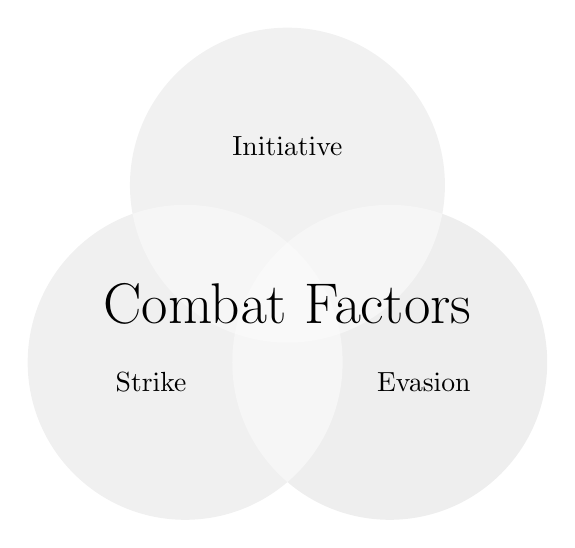
\begin{tikzpicture}
      \begin{scope}[blend group = soft light]
        \fill[gray!11!white]   ( 90:1.5) circle (2);
        \fill[gray!12!white] (210:1.5) circle (2);
        \fill[gray!13!white]  (330:1.5) circle (2);
      \end{scope}
      \node at ( 90:2)    {Initiative};
      \node at ( 210:2)   {Strike};
      \node at ( 330:2)   {Evasion};
      \node [font=\huge] {Combat Factors};
    \end{tikzpicture}}
}
%----

		\setcounter{track}{18}
		\posterbox{name=track,column=6,row=1,span=1,rowspan=12}{ 
			{\large

			\Repeat{18}{\tracker
			}


			}

			}


%----

\initblock{2}{2}

\initblock{2}{8}

\initblock{7}{2}

\initblock{7}{8}

%----

\end{tcbposter}

